\chapter{Background}
\label{chp:background}
\par This chapter provides an introduction to the technology behind \ac{IP} hopping and many of the previous efforts in this area. Section \ref{sec:routing} describes how routing at various points in a network works. Section \ref{sec:hopping} covers IP address space randomization---referred to as ``\ac{IP} hopping'' in this thesis---and the two possible approaches. Sections \ref{sec:data_security} and \ref{sec:totp} provide descriptions of two critical systems behind the implementation presented in this thesis, encryption and \ac{TOTP}. Finally, Section \ref{sec:related_research} examines previous effects in \ac{IP} address hopping.

\section{Network Routing}
\label{sec:routing}

\subsection{\ac{IP} Routing}
\label{sec:ip_routing}
\par This thesis makes the assumption that the reader has a famility with how \ac{IP} works. However, several aspects of this protocol are critical to the functioning of the system described later and are detailed here. 

\par Packets on the public Internet use \ac{IP} formatted-packets to communicate their source and destination. Two versions of this protocol exist, \ac{IPv4} and \ac{IPv6}, each with their own standardized header format. Table \ref{tbl:packet_structure} shows each of these headers.

\par \ac{IP} packets are routed from system to system based on the destination \ac{IP} contained in their header. IP version 4 uses 32-bit addresses to uniquely identify each system on the public Internet. These addresses are typically represented in a ``dotted quad'' format: for example, \texttt{74.125.228.36}. IP version 6 uses 128-bit address, typically represented in heximdecimal separated by colons (i.e. \texttt{a3d3:2d42::8c24}).

\begin{landscape}
\begin{table}
\caption{\ac{IP} Packet Structure \tbd{margins on this page...}}
\label{tbl:packet_structure}
\centering
\begin{tabular}{|c||c|c|c|c|c|c|c|c||c|c|c|c|c|c|c|c||c|c|c|c|c|c|c|c||c|c|c|c|c|c|c|c|}
\hline
	\multicolumn{33}{|c|}{\textbf{Packet Structure (32 bits wide)}}\\
\hline
	& 0 & 1 & 2 & 3 & 4 & 5 & 6 & 7 & 8 & 9 & 10 & 11 & 12 & 13 & 14 & 15 & 16 & 17 & 18 & 19 & 20 & 21 & 22 & 23 & 24 & 25 & 26 & 27 & 28 & 29 & 30 & 31\\
\hline
\hline
	\multirow{6}{*}{\rotatebox{90}{\textbf{IPv4}}}
		& \multicolumn{4}{|c|}{Version} & \multicolumn{4}{|c|}{Header Len} & \multicolumn{8}{|c|}{TOS} & \multicolumn{16}{|c|}{Len}\\
		\cline{2-33}
		& \multicolumn{16}{|c|}{ID} & \multicolumn{3}{|c|}{Frag Flags} & \multicolumn{13}{|c|}{Fragment Offset}\\
		\cline{2-33}
		& \multicolumn{8}{|c|}{TTL} & \multicolumn{8}{|c|}{Protocol} & \multicolumn{16}{|c|}{Header Checksum}\\
		\cline{2-33}
		& \multicolumn{32}{|c|}{Source IP}\\
		\cline{2-33}
		& \multicolumn{32}{|c|}{Destination IP}\\
		\cline{2-33}
		& \multicolumn{32}{|c|}{Options (optional, specified by header len)}\\
\hline
\hline
	\multirow{10}{*}{\rotatebox{90}{\textbf{IPv6}}}
		& \multicolumn{4}{|c|}{Version} & \multicolumn{4}{|c|}{Priority} & \multicolumn{24}{|c|}{Flow label}\\
		\cline{2-33}
		& \multicolumn{16}{|c|}{Payload len} & \multicolumn{8}{|c|}{Next header} & \multicolumn{8}{|c|}{Hop limit}\\
		\cline{2-33}
		& \multicolumn{32}{|c|}{\multirow{4}{*}{Source address}}\\
		& \multicolumn{32}{|c|}{}\\
		& \multicolumn{32}{|c|}{}\\
		& \multicolumn{32}{|c|}{}\\
		\cline{2-33}
		& \multicolumn{32}{|c|}{\multirow{4}{*}{Destination address}}\\
		& \multicolumn{32}{|c|}{}\\
		& \multicolumn{32}{|c|}{}\\
		& \multicolumn{32}{|c|}{}\\
\hline
\end{tabular}
\end{table}
\end{landscape}

\par Regardless of which version is in use, high-level routing remains conceptually the same. Routers maintain a table of \ac{IP} addresses, masks, and the interfaces associated with each. When a packet is received, the router consuluts this table and decides what interface to send the packet out on based on the most specific entry. For example, in the network shown in Figure \ref{fig:routing_example_network} the laptop with \ac{IP} 10.5.0.25 wants to send a packet to 172.100.10.3. When 10.5.0.25 sends its packet, the following sequence of events occurs:

\begin{figure}
\caption{Routing Example Network}
\label{fig:routing_example_network}
\centering
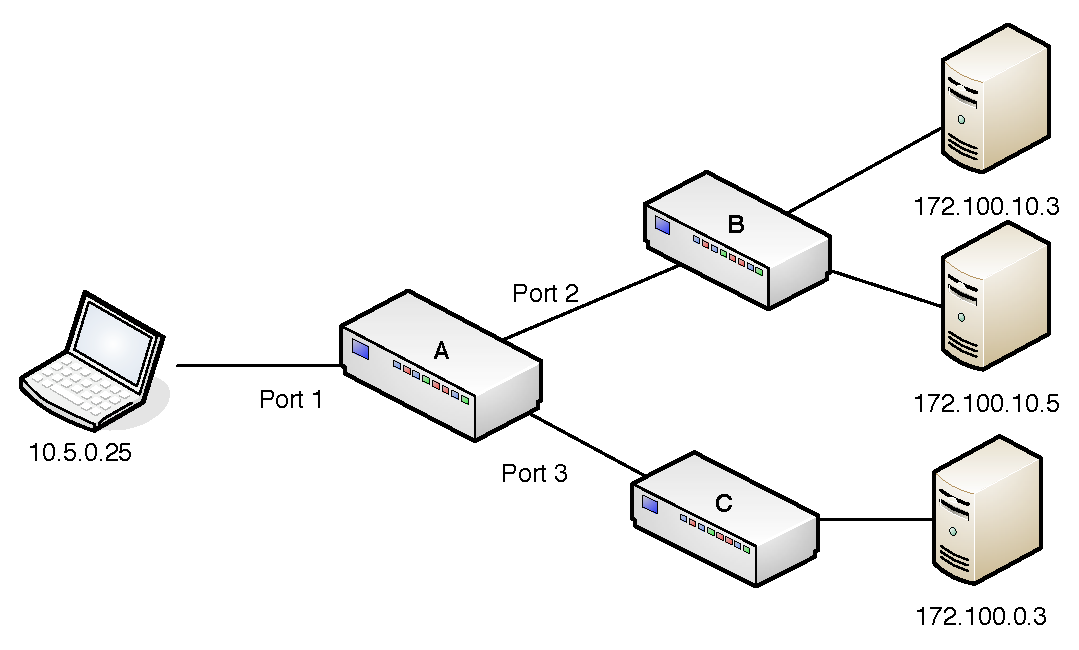
\includegraphics[width=1.0\textwidth]{routing_example_network.png}
\end{figure}

\begin{enumerate}[1.]
\item The packet leaves 10.5.0.25 and Router A receives it on its interface Port 1.
\item Router A pulls off the packet's destination \ac{IP} (172.100.10.3) and compares it to its table, which looks like Table \ref{tbl:routing_example_routera_table}.
	\begin{table}[h]
	\caption{Routing Example: Router A Table}
	\label{tbl:routing_example_routera_table}
	\centering
	\begin{tabular}{r|c|c|c}
	 & \ac{IP} & Mask & Interface\\
	\hline
	1 & 10.5.0.25 & 255.255.0.0 & Port 1\\
	2 & 172.100.10.0 & 255.255.255.0 & Port 2\\
	3 & 172.100.0.0 & 255.255.0.0 & Port 3\\
	\end{tabular}
	\end{table}
\item Router A determines the \ac{IP} matches best with entry 2, so it sends the packet out on Port 2.
\item Router B receives the packet and does a similar lookup, forwarding it out on the port to 172.100.10.3.
\end{enumerate}

\par This scheme allows a router to direct packets without having to know every individual IP; they only have to know broad swaths of addresses. In the example, Router A had no knowldege of how to get the packet directly to 172.100.10.3, but it did know which direction to send it. This becomes exponentially more useful on larger networks. A corporation's network, for instance, may contain hundreds or thousands of addresses, but the routers directing packets to them need only have one entry in their table to correctly route packets. The internal routers of the corporation are then in charge of further routing.

\par It is this limited-knowledge architecture that allows IP hopping to work. As long as the router's sending packets in cover the correct \ac{IP} ranges in their tables, the systems inside are free to change addresses as frequently as they want and handle internal routing any way they desire.

\subsection{Network Address Translation}
\label{sec:nat}
\par \ac{NAT} is core technology behind many modern home and corporate networks, allowing many systems to connect to the Internet yet appear to come from a single external \ac{IP} address. A typical home network, for instance, might have the external IP address \texttt{184.58.31.151} assigned to it by the \ac{ISP} yet have five systems---laptops, desktops, phones---inside with \acp{IP} like \texttt{192.168.0.103}, \texttt{192.168.0.50}, and \texttt{192.168.0.1}. As these systems send requests out, the router changes the source IP (and port) for packets to the external IP address. As responses come back from the Internet, the router does the opposite, changing the desitation of the packets from the external IP to the internal IP of the original requester.

\par To do this, routers must maintain a \ac{NAT} table. This table consists of the source and destination information as well as a new port number, allowing the router to consistently transform traffic in both directions. For example, a router might have a table like the one shown in Table \ref{tab:nat_example}.

\begin{table}
\caption{NAT Table Example}
\label{tab:nat_example}
\centering
\begin{tabular}{r|ccccc}
  & Int IP & Int Port & Remote IP & Remote Port & Ext Port\\
\hline
1 & \texttt{192.168.0.103} & 3547 & \texttt{74.125.225.69} & 443 & 50003\\
2 & \texttt{192.168.0.103} & 8751 & \texttt{207.109.73.34} & 80 & 42630\\
3 & \texttt{192.168.0.112} & 30452 & \texttt{4.27.2.253} & 80 & 53920
\end{tabular}
\end{table}

\par This small table shows three different connections in progress. The router created each entry the first time the interal system sent out a packet to the remote (Internet) one, for each set of internal and remote IPs and ports. In addition, the router assigns an external port for each connection to allow it to determine to whom incoming packets are destined.

\par In the future, when the router receives an outgoing packet (from the interal host to the exteral), it begins by consulting its table to find a match based on the first four values in the table. Assuming it finds a corresponding entry, the router changes the source IP of the packet to the exteral IP assigned to it by the \ac{ISP} and the source port to the external port given in the table. When the router receives a packet from the Internet, it checks for a match in the table based on the remote IP, remote port, and external port. If it finds one, it alters the packet's destination information to the internal IP and port.

\par This system serves two purposes. First, as the number of systems on the Internet has increased, \ac{IPv4} addresses have become a precious resource, with their 32-bit length limiting the number of possible addresses to around four billion. \ac{NAT} allows an organization to only own a single address yet serve many systems behind it. Second, \ac{NAT} inherently acts a simple stateful firewall. In order for an outside system to send packets to an internal host, the internal host must have initiated the connection and allowed the router to create the table entry.

\subsection{Ethernet and \acf{ARP}}
\label{sec:eth_routing}
\par Many local networks use Ethernet for the last leg of network travel to actual hosts. In a flat network, where local machines are connected together via a switch or hub, \ac{IP} routing is not typically used. Instead, packets are directed to the correct recicient via physical identifiers known as \ac{MAC} addresses. Packets sent on an Ethernet network are wrapped in an Ethernet frame, which specifies the \ac{MAC} addressses of the sender and receiver.

\par When a packet is first created, however, the host system only knows the destination \ac{IP}. Before the packet can be sent out, the destination \ac{MAC} address must be determined. This is done through a \ac{ARP} request, a process illustrated in Figure \ref{fig:arp_example}.

\begin{figure}[ht]
\caption{\ac{ARP} Example}
\label{fig:arp_example}
\centering
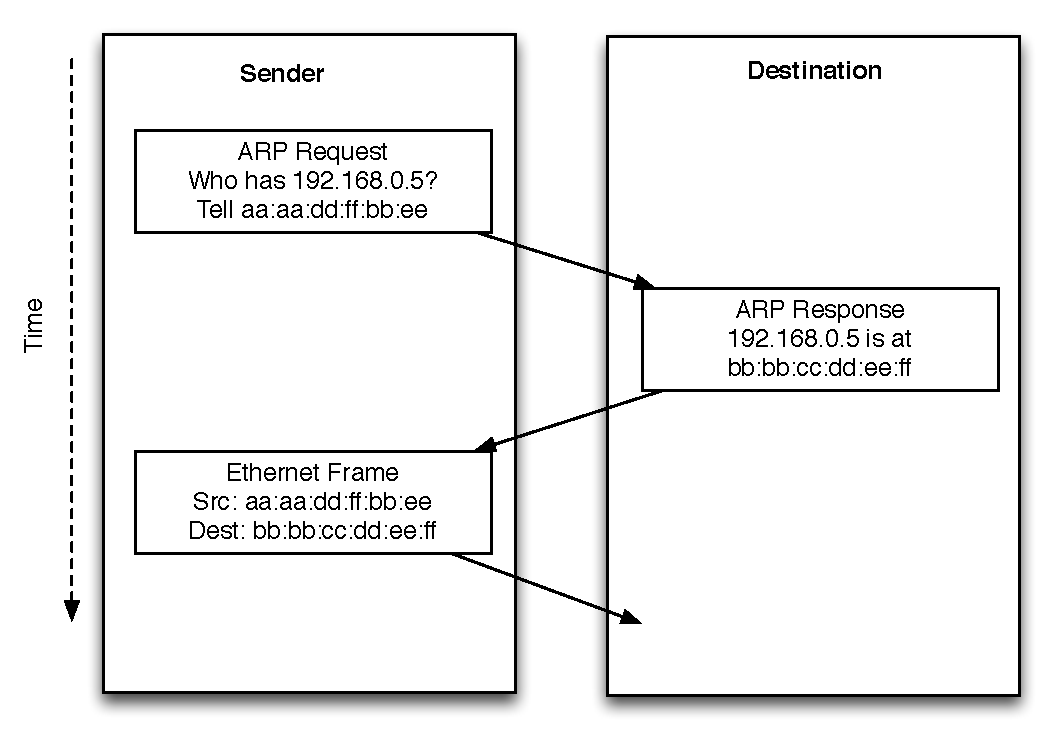
\includegraphics[width=0.8\textwidth]{arp}
\end{figure}

\par As shown, the sender first asks on the network who has the destination \ac{IP}. Every host on the network hears the request, but only the one with that \ac{IP} responds, sending back an \ac{ARP} response with their \ac{MAC} address to the requster. With the destination \ac{MAC} now in hand, the original sender can contruct the Ethernet frame for their \ac{IP} packet and send the data on its way. The sender caches the physical address of the other machine for a short time to avoid repeating the \ac{ARP} request too frequently.

\section{IP Hopping in Detail}
\label{sec:hopping}
\par Address hopping is a simple concept at a high level: take the basic identifiers of a network and mutate them in a way that only authorized systems can follow. Doing so makes it difficult for an adversary to correlate sniffed traffic with individual machines and even more difficult to probe into the network to enumerate hosts. In trying to actually implement such a system, however, several issues arise. 

\par The network illustrated in Figure \ref{fig:exnetwork} is used to aid the following discussion. There are two main networks \textit{A} and \textit{B} that are assigned the displayed IP ranges, are connected by the Internet, and have an interest in communicating freely with one-another. Each of these has a few friendly end nodes (\textit{A1}, \textit{A2}, etc) behind a main router (\textit{AR} and \textit{BR}). Additionally, network \textit{B} has a potentially rogue client inside it named \textit{M1}. Outside of those two networks is the friendly \textit{C2} node, who has an interest in at least occasionally communicating with nodes inside \textit{A}/\textit{B}, and malicious \textit{M2}, who wants access to said networks. The details of the routes between them and \textit{A} and \textit{B} are inconsequential.

\par Note that for the sake of this discussion non-routable \ac{IPv4} addresses are largely used. This is done merely for convenience and readability, the discussions apply to \ac{IPv6} as well unless otherwise noted.

\begin{figure}
	\centering
	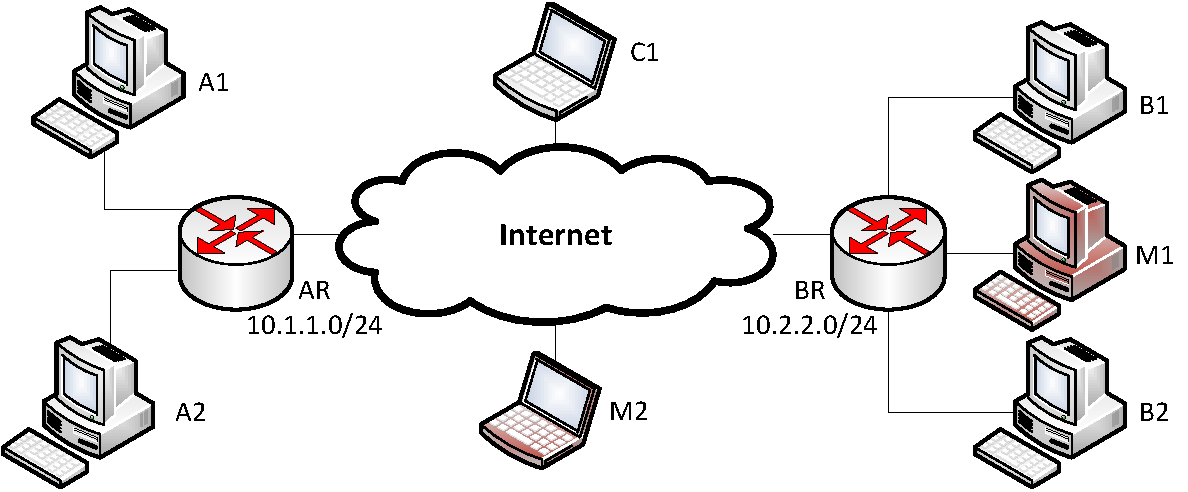
\includegraphics[width=0.75\textwidth]{exnetwork}
	\caption{Example network layout \tbd{include IP addresses}}
	\label{fig:exnetwork}
\end{figure}

\par There are two basic ways IP address hopping could be deployed on this network: each end point hops individually or the network gateways transform incoming and outgoing packets. Both options and their strengths and weaknesses are discussed below.

\subsection{End Point Hopping}
\par For the example network, each end point hopping would mean that all of the nodes behind \textit{AR} and \textit{BR} (\textit{A1}, \textit{A2}, \textit{B1}, etc.) change addresses on a periodic basis, independent of one another. Despite the apparent simplicity of this setup, several questions must be answered.

\par First, how do the nodes keep track of one another? If every node knows about all the others, then scalability might become an issue, as every client presumably has to maintain some amount of data on fellow hopping clients to determine where each one is at any given time. It may be possible to devise a scheme where this flaw is mitigated by having all clients hop using the same secret and they each know just the broad IP ranges where fellow hoppers reside (i.e., the \textit{AR} nodes know that 10.2.2.0/24 is a network they talk to with hopping), but this accentuates the next question: how do clients choose their hops?

\par Clearly, each node must know some secret from which IP addresses are generated, hopefully in a manner which appears random to outsiders yet is predictable for those with the secret (the ``hopping pattern''). There may be only one of these secrets, which every node in the protected network knows---that is, the nodes in both A and B, hereafter collectively referred to as the ``hopping network.'' This does have the potential flaw of revealing too much information to an eavesdropper though: with a large number of nodes all following a hopping pattern based on the same key, it may be easier to deduce the secret.

\par Giving each node a separate secret would solve this issue. However, each client now has to maintain even more information on every other client. For a small number of nodes this is not a problem, but if the intention is to scale to the thousands or tens of thousands problems with processing and key distribution may arise.  

\par Just as importantly, however, is the question of how nodes coordinate their IP address choices. As discussed in Section \ref{sec:routing}, IP routing requires addresses follow a largely hierarchical setup, with broad ranges like 10.0.0.0 leading to 10.1.0.0 to 10.1.1.0 and so on. Thus, if \textit{A} has the network address range 10.1.1.0/24, then all of its nodes must fall within the address range of 10.1.1.1 through 10.1.1.255. This means that when each node hops it must remain within the valid range of the network it is a part of \textit{and} that the address it chooses must not already be taken another node. Given enough nodes in a subnet, a conflict is quite possible, leading to unpredictable network behavior. 

%\par It is likely possible to devise a reasonably robust algorithm for all nodes to hop simultaneously and end up on unique IPs, but this encounters a few issues with the link-layer of a network's architecture. On local networks, machines are identified by a Media Access Code (MAC) and systems must map IP addresses to the hardware MAC using Address Routing Protocol (ARP). Nodes virtually always cache this information for speed, so for the period of time from a hop to the cache entry expiration time, packets sent to nodes on the local network will likely contain an incorrect MAC and not arrive at the correct destination. TCP would then detect the packet loss and retransmit, trying until either the connection timed out or the ARP cache updated. Even if ARP information is only cached for a few seconds, at best this could result in bursts of traffic on local networks and at worst dropped connections. A similar problem also exists at the switches in the network, although this would likely resolve itself quickly.

%\par It would be possible to work around this issue by having whatever utility is handling the hopping also alter the ARP cache. To do so, every node would need to compute the correct locations of all other nodes and do so at precisely the same time. While not infeasible, this becomes even more platform-specific than the general IP hopping was. Approaching it the other way, nodes could all send gratuitous ARPs when their IP changes, but this still generates extra traffic on the network and \textit{forces} systems to be extremely vulnerable to ARP spoofing, a common part of a network attack.

\par The easiest solution to this problem is to give each node a unique, non-overlapping address range in which to hop. This requires no on-going communication with other nodes to work well and has the distinct advantage of working properly with existing defenses (i.e., a firewall with special rules for a host can point to the range for that host, rather than an individual IP). This setup poses the potential difficulty of requiring a large enough address space to make hopping beneficial. If a given node only has five possible addresses in which to hop, for instance, it becomes trivial for an attacker to just keep trying a single one until the node returns to it. \ac{IPv6} would aleviate this problem, as the Internet Engineering Task Force recommends the allocation of a /64 address space ($2^{64}$ addresses) to every link \cite{rfc3267}, but \ac{IPv4} with its more limited address space would not allow this flexibility and, unfortunately, the reality of current networks mandates support for \ac{IPv4}. \tbd{see if a paper has an analysis of the needed address space for usability}

\par Of course, with enough coordination between nodes everyone could share the same address space. A fair amount of work would need to be put into an algorithm and protocol to synchronize everyone's changes, but this is not insurmountable. This does break most special cases in firewalls unless the firewall is either made aware of the \ac{IP} hopping system or hosts that need special rules do not change addresses at all.

\par Despite these negatives end point hopping does have advantages. First, scalability issues lie more in storage space and key lookup speed than actual computation, as every node only has to perform packet transformations for their own ingress and egress packets. Although not discussed yet, it is likely that any IP hopping scheme will also incorporate packet encryption, so distributing this load may be beneficial. Second, end point hopping protects clients from probing no matter where the adversary is in the network. For example, as long as \textit{M1} in our example network lacks the hopping key, they have no more of an advantage in scanning any of the \textit{A} or \textit{B} nodes than \textit{M2}, who is outside the network. Finally, end point hopping comes with the ability for individual nodes such as \textit{C1} to connect to the main hopping network, without requiring any additional work or software development.

\subsection{Gateway hopping}
\label{sec:gateway_hopping}
\par The alternative to end point hopping is to move the hopping to network gateways. In such a scheme, networks are placed behind gateways that alter all traffic passing through them appropriately. What ``appropriately'' means varies with every implementation, but in one way or another, a gateway outside of the actual end points alters the IP traffic to make it appear as though the systems inside are changing IP addresses. Referring back to the example network in Figure \ref{fig:exnetwork}, gateways \textit{AR} and \textit{BR} would be in charge of these packet transformations, altering traffic from the clients inside their networks (e.g., \textit{A1}, \textit{A2}, etc.) to outsider hosts. The secrets that were used at the end point level before are now stored at the gateway, although it is usually concentrated down to per-gateway level granularity; the gateways have no precise knowldge of the end points they protect.

\par Nodes inside the network may or may not have knowledge of the hopping. In most instances the hopping occurs with no modification of the end points and is largely transparent. \tbd{cite} This need to only deploy a small number of systems, rather than altering every system, gives gateway-based hopping an advantage over end point-based on larger networks. Applying software and/or hardware changes to every system is costly in terms of both time and manpower. Even more significantly, legacy systems running older operating systems would likely need custom solutions and might be completely unsupportable as a result.

\par The most common observable side effect of gateway hopping (beyond the latency associated with the additional processing) is \ac{TCP} connection dropping \tbd{cite. Really need to re-read all the papers}. Because TCP depends on IP addresses and ports numbers to identify on-going connections, any alterations to this information would traditionally kill the connection. This is a problem also faced by end point hopping schemes, but is more easily corrected because the individual machines know the state of connections and can correct appropriately. With gateway hopping, however, the situation may require significant state tracking at the gateway.

\par Because of this required state tracking and the need for a single system to alter all traffic in and out of an entire network, gateway-based hopping presents a possible performance problem. With enough traffic or individual nodes behind a gateway, it may be possible to overload the gateway, leading to dropped packets and failing connections. Depending on gateway design this may be avoided; some studies show a CPU impact of around 10\% (even when encryption is applied) when compared to plain routing \cite{TAO}.

\par Additionally, gateway hopping may have more difficulty accomodating individual clients connecting to the network. In \textit{C1}'s case, for instance, if it wanted to be able to talk to \textit{A1}, it would need to obtain the appropriate hopping information from \textit{AR} and alter its own traffic accordingly. There are several ways to make this work, but all of them require more work than an end-point hopping system would, simply because end-point hopping was already designed around the concept of individual nodes connecting together.

\section{Data Security}
\label{sec:data_security}

\subsection{Hashing}
\label{sec:hashing}
\par Cryptographic hash functions take a given sequence of bytes and return a fixed-length string of bits representing that data. While not their output is not unique for every input, crytographic hashes attempt to make it infeasible to generate two messages with the same hash or to modify an input and get the same hash. As illustrated in Table \ref{tbl:hashing_example}, these properties allow the use of hashes in to verify data because even small changes result in different output.

\begin{table}[h]
\caption{Hashing Example}
\label{tbl:hashing_example}
\centering
\begin{tabular}{r|l|l}
	& Input & Output (SHA-1)\\
\hline
Original & The quick brown fox jumped & c950af1b07223c7d8590538189b3bcd9f4e08c6c\\
Changed & The quick br\textit{\textbf{a}}wn fox jumped & 97c592d5c0d991b91c68edb3941b1bb075a97f56
\end{tabular}
\end{table}

\par Here even a small change (\textit{o} to \textit{a}) resulted a significantly different output. If the sender gave both the data and the hash to a recipient, the recicipent would be able to repeat the hash on the data and verify that their hash matches the one the sender gave them. Of course, hash algorithms like \ac{SHA} (used in this example) are widely published, so anyone can produce a valid hash of any data they want. This means that in and of themselves, hashes do not prevent against malicious modification: an attacker could modify data, then produce a new hash to match. To work around this problem, a digital signature or \ac{HMAC} must be used, as covered in Section \ref{sec:authentication}.

\subsection{Encryption}
\label{sec:encryption}
\par As is discussed in Section \ref{sec:related_research}, encryption is a crucial component of most hopping systems. Additionally, encryption forms the basis of digital signatures and \ac{HMAC}, both means of verifying that a given message---a single packet, in most contexts here---came from where the receiver believes. It is not important for the purposes for this thesis to understand the math behind encryption, but a few concepts are helpful.

\par Encryption comes in two major flavors, symmetric and asymmetric. Symmetric encryption uses the same key for encryption and decryption and, in many cases, is fairly quick. Newer \acp{CPU}, such as Intel's Core processors, include hardware instructions for the commonly used \ac{AES} algorithm, increasing symmetric encryption's speed even further \cite{IntelAES}. Because anyone with the encryption key can decrypt the data, participants must establish their shared secret in a secure way.

\par Asymmetric encryption---also preferred to as public-key encryption---provides a way to exchange secure data \textit{without} having to establish a secret key beforehand. In asymmetric encryption a public key---known to everyone---and a private key---known only to one participant---are used in conjunction. If a sender wants to transmit data to a specific receiver securely, they encrypt the data with the receiver's public key. When the receiver gets the transmission, they decrypt it with their private key. Because no one else knows the private key of the receiver, it is impossible for anyone else to decrypt the data, even though the encryption key is widely known. In exchange for the robustness and openness of this encryption style, asymmetric encryption algorithms tend to be slow.

\par Asymmetric and symmetric encryption are typically used together in network communications. When a connection is first established, a public-key encryption scheme such as \ac{RSA} determines the shared symmetric key, then all future data is encrypted with a symmetric algorithm like \ac{AES} \cite{HybridEncryption}. This hybrid approach provides the best of both worlds: no need to establish a shared secret in advance and speed during longer communications.

\subsection{Authentication}
\label{sec:authentication}
\par Authenticating that a given sequence of bytes actually comes from whom they say they do can be done through either a \ac{HMAC} \cite{rfc2104} or a digital signature \cite{rfc3447}. These alorithms are based an symmetric and asymmetric encryption, respectively, and therefore share the same strengths and weaknesses. Again, the exact details of the math and operation behind these algorithms is irrelevant for the purposes of this thesis. 

\par Both algorithms essentially work by encrypting a hash of the data being sent and verifying that hash on the receiving side. In the case of \ac{HMAC}, both ends have the same shared private key, so they each do the \ac{HMAC} process independently and the receiver ensures their calculated HMAC matches the one sent with the message. If it does, the receiver knows the message is unchanged and comes from someone with the correct shared key.

\par For a digital signature, the sender encrypts the hash with their own private key. The receipient verifies the authenticity of the message by performing their own hash of the data and decrypting the signature with the sender's public key. If the calculated hash and the decrypted hash match, the sender must be who they claim to be, as only that sender has access to the correct private key.

\subsection{Combining for Full Effect}
\label{sec:auth_and_encrypt}
\par By combining encryption and authentication, two parties can communication with confidentiality and integrity. For public key encryption, a sender signs the message with their own private key, then encrypts the message with the public key of the recicient. The recicient decrypts the message with their private key, then verifies the signature with the public key of the sender.

\par For symmetric encryption, the opposite order is used. First the sender encrypts the data with one symmetric key, then adds an \ac{HMAC} of the ciphertext \cite{AuthEncrypt}. The receiver computes the \ac{HMAC} of the cipher text and verifies the attached one to ensure the integrity and authenticity of the message. The receiver then decrypts the data.

\section{\acf{TOTP}}
\label{sec:totp}
\par The system discussed in this thesis relies heavily on values that are unpredictable to an outsider but calculatable for anyone with the secret key. The algorithm behind these values is \ac{TOTP} \cite{rfc6238}, which in turn relies on the \ac{HOTP} algorithm \cite{rfc4226}. Both of these algorithms are frequently used in the two-factor authentication systems employed by banks and other websites, with a smartphone app or key fob displaying the current password.

\par \ac{HOTP} utilizes a key of at least 128-bits and a ``counter'' to produce its output. These passed to a \ac{SHA}-based \ac{HMAC}, which produces a 20-byte string. It then applies a ``truncation'' process to the \ac{HMAC}, finally returning a four-byte output \cite{rfc4226}. If both sides of an exachange know the key and the current counter, they are able to indepently produce the same value.

\par The counter for \ac{HOTP} is set based on some event that the system designer decides upon. In the most literal case, the usage of a given output for authentication causes an internal counter to be incremented. In a situation like this, both sides of the HOTP (the sender and the receiver) must keep their counters in-sync or the two will produce differing values and need to be resynchronized. In a system with multiple senders and receivers, this becomes quite challenging.

\par To work around this, time may instead be used as the basis of the counter. RFC 6238 defines \ac{TOTP} as a simple extension of \ac{HOTP} where the counter becomes the current time divided by a configured time step \cite{rfc6238}. This change allows all parties interested in a given \ac{TOTP} to produce the same value as long as they keep their clocks relatively similar (within one time step). 

\section{Previous Implementations}
\label{sec:related_research}

\tbd{present-tensify}

\subsubsection{BBN's \acf{DYNAT}}
\par In 2001, BBN Technologies released a paper entitled ``Dynamic Approaches to Thwart Adversary Intelligence Gathering'' \cite{BBNDYNAT}. In this paper, they set out to test the hypothesis that ``dynamic modification of defense structure improves system assurance.''

\par Their \ac{DYNAT} technique, as they called it, was put through a series of red-team experiments to test if it decreased an adversary's ability to map the network. The experimentation confirmed BBN's hypothesis: DYNAT did in fact increase system assurance because the adversary's work greatly increased compared to static networks. Even when the red team was given intimate knowledge of DYNAT's operation, the adversary could not identify a critical server in an enclave with DYNAT active.

\par The BBN's DYNAT implementation focused on individual clients connecting to a server enclave, through a DYNAT gateway on the server end. This gateway transformed incoming and outgoing packets between ``true'' host identification information---e.g., the actual IP address and port number of a server inside the enclave's network---and values which varied based on a pre-shared key and time. On the client side, a ``DYNAT shim'' sat in the network stack and did the same thing, transparently allowing client applications to work with the server enclave. Additionally, DYNAT applied encryption to all traffic for confidentiality.

\par BBN's experiments also demonstrated that the encryption of the packets was critical, as the attackers could trivially sniff the traffic to find important servers, even if they did not know the real IP address or port of the target. For example, an attacker could see a packet contained an \ac{HTTP} response and thus learn an active IP and port for a web server, even if probing for it was impossible. While this information would only be valid for a limited period, it may be enough time for the attacker to compromise the internal network.

\subsubsection{Sandia Dynat}
\par In 2002, Sandia National Labs released a final report on their extensive work in the ``dynat'' field \cite{SandiaDynat}. This report covers virtually every variable in a dynat system, from how hopping is synchronized to where in the network it is implemented. This paper points to many of the important issues that must be considered when implementing or deploying a dynat.

\par Of particular importance to our implementation proposal (ARG) are Sandia's recommendations on the location of the deployment of a gateway-based dynat. In order to avoid interference with existing firewall rules---particularly ones with a stateful firewall---, a dynat must be deployed beyond the current system. Likewise, for gateway-based virtual private networks (VPN), there is often a static IP requirement to allow for authentication \cite{SandiaDynat}, so a IP hopping gateway must also lie beyond the VPN concentrator. Essentially, the hopping gateway should be the last system before each the network connects to the outside world \cite{SandiaDynat}.

\par The Sandia report also provides significant insight into the interaction of a dynat with IPSec and strongly suggests a combination of the two. First, the encryption from IPSec avoids the ineffectiveness of dynat if the packets can be trivially sniffed for information, as already discussed in \cite{BBNDYNAT}. Second, IPSec is strengthened with the addition of a dynat, as the dynat can quickly reject invalid packets based on invalid source and destination identifiers, rather than forcing IPSec to perform expensive HMAC computations and/or encryption. However, the report also warns that the use of IPSec with dynat can reduce some aspects of dynat's access control because more identifiers are encrypted and unusable.

\subsubsection{\acf{APOD}}
\par In 2003, BBN proposed another IP hopping implementation as part of the \ac{DARPA} \ac{APOD} project \cite{APOD}. This system was a refined version of the previous BBN DYNAT, featuring a \ac{NAT} gateway sitting either on the server host itself or on a gateway into the network.

\par As noted by the authors, the primary differences between APOD and the previous DYNAT related to implementation. Whereas the BBN DYNAT was a very specialized solution, APOD employed standard \ac{COTS} utilities, such as Linux's iptables, to perform much of its work. They furthermore noted that APOD could be implemented as a NAT gateway on the networks of both the client and the server.

\subsubsection{\acf{NASR}}
\par The 2005 \acf{NASR} was an IP address hopping system designed to defeat hitlist-based worms \cite{NASR}. These worms spread to pre-collected lists of IP addresses and typically propagate much faster than traditional worms that target random IPs. To fight this, NASR caused the pre-built hitlists to decay by changing IP addresses on a periodic basis.

\par The most unique aspect of this research was the use of \ac{DHCP} to force the changes. Through the use of a slightly intelligent \ac{DHCP} server that leased \acp{IP} for a only a short time frame (on the order of tens of minutes) and only offered IPs that have not been used recently, most networks already using DHCP can be quickly changed to a randomized scheme. This simplicity does come at a cost, however: TCP connections are killed whenever the IP change occurs, forcing the hopping period to be quite long or risk unacceptable connection losses. The researchers did introduce intelligence into the DHCP server to allow it to detect ``long-lived'' TCP connections (i.e., a download) and give clients the same IP if they appeared busy. Beyond that, they also monitored what services a client was using, as many are resilient to a connection being torn down \cite{NASR}.

\par Despite those improvements, address changes occurred even in the fastest of instances only once an hour or so. This met the goal of hitlist worm protection, but is likely inadequate for obfuscating the network from a more intelligent enemy.

\subsubsection{\acf{NAH}}
\par In 2005, European researchers presented a system they named \acf{NAH} \cite{NAH}. This system focused on a client contacting a server as a negotiable protection measure, rather than an always-on system used between pre-configured systems.

\par A protocol employing \ac{IPv6} allowed a client to tell a server that they supported (and wished to use) NAH. If the server supported NAH, it replied with its hopping pattern. The client then sent its own hopping pattern, before reconnecting using the pattern the server just gave it. Packet count per connection was used to synchronize the hops and detect lost packets.

\par Once again, the NAH authors noted that encryption was important to maintaining the confidentiality of the data stream. However, they also stated that without encryption the system still provided some benefit, as packets bound for ``different'' addresses might follow differing routes due to the different (perceived) destinations. This means an attacker would need to either compromise a route fairly close to an endpoint to ensure they saw all traffic or compromise every possible route and collate the traffic together. Even if they manage to accomplish that, the attacker would still have to collect all traffic passing them in order to reconstruct the full stream (because they are unable to filter for specific IPs to identify the connection they are interested in), which poses a storage and computation problem given enough data \cite{NAH}.

\par As an additional side effect of the variable routing, the researchers noted that such a system may actually increase the throughput and reliability of a system. If multiple routing paths are used, congestion may be avoided and traffic ultimately flows more smoothly \cite{MultimediaDistributed}. While this is not viewed as an important aspect of this system, the potential does add support to the employment of address hopping.

\subsubsection{\acf{TAO}}
\par Finally, in 2006 a system called \ac{TAO}(TAO) was proposed \cite{TAO}. This system focused on protection of the Internet as a whole from hitlist-based worms and was somewhat based on the previous work in \ac{NASR} \cite{NASR}. It featured gateways on networks that maintained external-to-internal address mappings for all nodes inside the protected network, with the external addresses changing with a configurable frequency. To maintain existing connection regardless of mapping changes, TAO included a \ac{NAT} table. 

\par A disadvantage of this design was address space overhead. Testing showed that around 10\% more address space was needed for three simulations on large-scale networks, based on the need to reserve addresses to maintain connections while continuing to change address mappings. However, TAO had the distinct advantage of only requiring the addition of a single box at the network's edge and no cooperation from remote hosts was needed for it to provide its services.

\tbd{include CONTRA?}

